% TeleCon4ESP32 user guide — Android application for makers.
% Build: pdflatex -output-directory=../build telecon_user_guide.tex
\documentclass[12pt,a4paper]{article}

\usepackage[margin=2.4cm]{geometry}
\usepackage[T1]{fontenc}
\usepackage[utf8]{inputenc}
\usepackage{lmodern}
\usepackage{booktabs}
\usepackage{hyperref}
\usepackage{xcolor}
\usepackage{colortbl}
\usepackage{array}
\usepackage{enumitem}
\usepackage{needspace}
\usepackage{etoolbox}
\usepackage{tikz}
\usepackage{graphicx}
\usepackage{float}
\usepackage{caption}
\captionsetup{justification=centering,singlelinecheck=false}

\usetikzlibrary{arrows.meta,shadows}
\preto\section{\Needspace{9\baselineskip}}

\hypersetup{
  colorlinks=true,
  linkcolor=black,
  urlcolor=blue,
  pdftitle={TeleCon4ESP32 User Guide},
  pdfauthor={TeleCon}
}

\definecolor{ArduinoKeyword}{HTML}{00979C}
\definecolor{ArduinoFunc}{HTML}{D35400}
\definecolor{ArduinoComment}{HTML}{5D6D6E}
\definecolor{ArduinoPreproc}{HTML}{9B59B6}
\definecolor{TblHead}{HTML}{0F6F73}
\definecolor{TblSync}{HTML}{E8DAEF}
\definecolor{TblChan}{HTML}{D5F5E3}
\definecolor{TblKnob}{HTML}{D6EAF8}
\definecolor{TblSw}{HTML}{FCF3CF}
\definecolor{TblSum}{HTML}{FAD7A0}
\definecolor{TblEnd}{HTML}{E5E7E9}
\definecolor{TblTelem}{HTML}{D4E6F1}
\definecolor{TblId}{HTML}{F5CBA7}
\definecolor{WireApp}{HTML}{0F6F73}
\definecolor{WireBg}{HTML}{F4FBFC}

\newcommand{\thc}[1]{\textcolor{white}{\bfseries #1}}
\newcommand{\chip}[2]{\colorbox{#1}{\strut\,\scriptsize #2\,}}
\newcommand{\ui}[1]{\textsf{\textbf{#1}}}

\tikzset{
  telecon actor/.style={
    rounded corners=4pt, minimum width=2.7cm, minimum height=1.05cm,
    font=\sffamily\bfseries, text=white, inner sep=4pt
  },
  telecon step/.style={
    circle, inner sep=1pt, minimum size=0.52cm,
    font=\sffamily\bfseries\scriptsize, text=white
  },
  telecon pill/.style={
    rounded corners=2.5pt, inner sep=3.2pt,
    font=\sffamily\scriptsize, align=center
  },
  telecon arr/.style={-{Latex[length=2.1mm]}, line width=0.9pt}
}

% Prefer figures/en/<file>, then shared figures/<file>.
\newcommand{\shotlang}{en}
\newcommand{\shotimg}[1]{%
  \begin{tikzpicture}
    \node[inner sep=0] (img) {%
      \phantom{\includegraphics[width=0.68\textwidth,height=0.48\textheight,keepaspectratio]{#1}}%
    };
    \fill[black, fill opacity=0.12, rounded corners=13pt]
      ([xshift=-5.5pt+1.8mm,yshift=-5.5pt-2.3mm]img.south west) rectangle
      ([xshift=5.5pt+1.8mm,yshift=5.5pt-2.3mm]img.north east);
    \fill[black!92, rounded corners=13pt]
      ([xshift=-5.5pt,yshift=-5.5pt]img.south west) rectangle
      ([xshift=5.5pt,yshift=5.5pt]img.north east);
    \begin{scope}
      \clip[rounded corners=10pt]
        (img.south west) rectangle (img.north east);
      \node[inner sep=0] at (img.center) {%
        \includegraphics[width=0.68\textwidth,height=0.48\textheight,keepaspectratio]{#1}%
      };
    \end{scope}
    \draw[black!30, line width=0.65pt, rounded corners=13pt]
      ([xshift=-5.5pt,yshift=-5.5pt]img.south west) rectangle
      ([xshift=5.5pt,yshift=5.5pt]img.north east);
    \draw[TblHead, line width=1.25pt, line cap=round]
      ([xshift=-5.5pt+11pt,yshift=-5.5pt+3.4pt]img.south west) --
      ([xshift=5.5pt-11pt,yshift=-5.5pt+3.4pt]img.south east);
  \end{tikzpicture}%
}
\newcommand{\shot}[4]{%
  \par\addvspace{0.25em}%
  \IfFileExists{../../figures/\shotlang/#2}{%
    \begin{figure}[H]
      \centering
      \shotimg{../../figures/\shotlang/#2}%
      \caption{\textbf{#1.} #4\\[0.35em]
        {\sffamily\scriptsize\color{ArduinoComment}#3
          \enspace\textbullet\enspace\texttt{\detokenize{#2}}}}
    \end{figure}%
  }{%
    \IfFileExists{../../figures/#2}{%
      \begin{figure}[H]
        \centering
        \shotimg{../../figures/#2}%
        \caption{\textbf{#1.} #4\\[0.35em]
          {\sffamily\scriptsize\color{ArduinoComment}#3
            \enspace\textbullet\enspace\texttt{\detokenize{#2}}}}
      \end{figure}%
    }{%
      \noindent
      \begin{tikzpicture}
        \node[
          draw=TblHead, fill=TblSw, line width=1.15pt, rounded corners=6pt,
          inner sep=10pt, text width=\dimexpr\linewidth-22pt\relax, align=left
        ] {
          {\sffamily\bfseries\color{TblHead} Screenshot #1
            \hfill{\normalfont\ttfamily\scriptsize \detokenize{#2}}}\\[0.35em]
          {\sffamily\scriptsize\color{ArduinoFunc} #3}\\[0.45em]
          {\sffamily\small #4}\\[0.35em]
          {\sffamily\scriptsize\color{ArduinoComment}
            Save as \texttt{General\_Documentation/figures/en/\detokenize{#2}} (or shared \texttt{figures/}).}
        };
      \end{tikzpicture}%
    }%
  }%
  \par\addvspace{0.2em}%
}


\title{TeleCon4ESP32 User Guide\\[0.35em]
\large Phone app for Control Panel and RC Vehicle}
\author{For people who use the Android application\\
\small Firmware authors: see the Control Protocol PDF}
\date{Version 1.0 \quad 2026}

\begin{document}
\maketitle

\begin{abstract}
This guide is for the person holding the phone.
It shows how to install TeleCon4ESP32, flash a starter ESP32 sketch, connect,
and drive \ui{Control panel} or \ui{RC Vehicle}.
Byte formats, UUIDs, and checksums live in the Control Protocol document.
Per-sketch pinouts and Serial banners live in that sketch's user guide.
\end{abstract}

\section{What TeleCon is}
\label{sec:what}

The phone is always the remote.
The board (ESP32 DevKit, ESP32-CAM, or any MCU that speaks the contract) is
the machine.

Two modules ship today:

\begin{center}
\renewcommand{\arraystretch}{1.25}
\begin{tabular}{>{\raggedright\arraybackslash}p{3.4cm}
                >{\centering\arraybackslash}p{2.2cm}
                >{\raggedright\arraybackslash}p{6.6cm}}
\rowcolor{TblHead}
\thc{Module} & \thc{Access} & \thc{What you do with it} \\
\rowcolor{TblChan}
\ui{Control panel} & FREE & Dual sticks, switches, knobs, gauges, and plots
for any ESP32 project. \\
\rowcolor{TblSum}
\ui{RC Vehicle} & PRO / coins & Driving cockpit plus optional ESP32-CAM video. \\
\end{tabular}
\end{center}

\vspace{0.4em}
{\sffamily\scriptsize
\chip{TblChan}{Control panel --- free}
\chip{TblSum}{RC Vehicle --- Pro}
\chip{TblTelem}{Video is a separate Wi-Fi link}}

Both modules share the same control session.
Camera video (HTTP \texttt{/stream}) is a second link: join the board's Wi-Fi
for pictures; Bluetooth or TCP carries sticks.

\Needspace{11cm}
\begin{center}
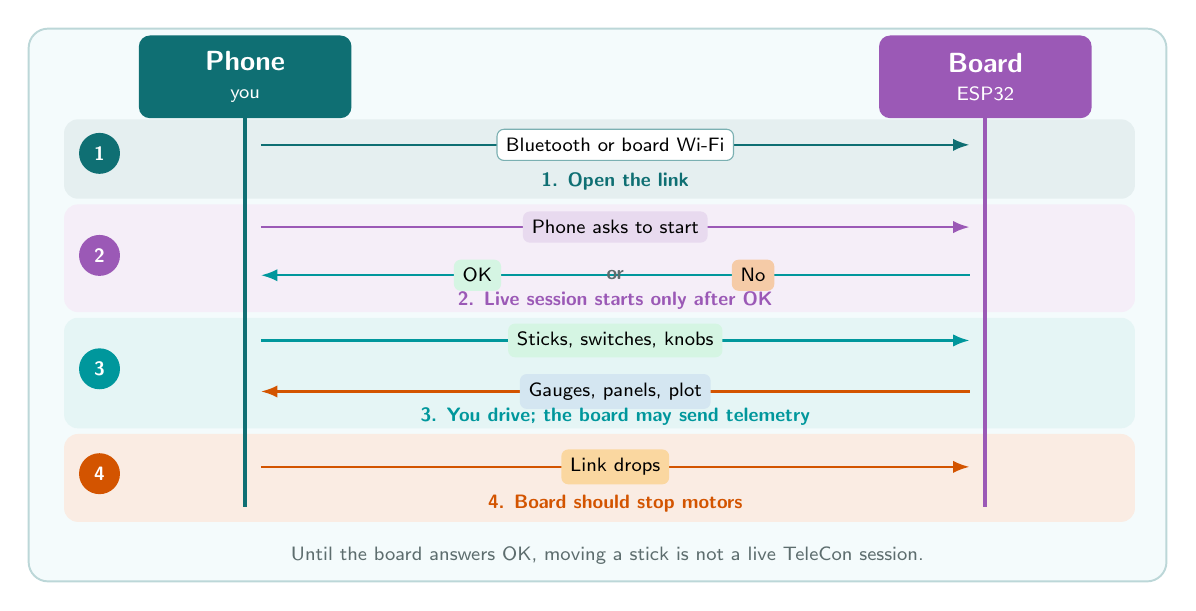
\begin{tikzpicture}[x=1cm, y=0.72cm]
  \fill[rounded corners=7pt, WireBg] (-0.35,-1.2) rectangle (14.1,8.55);
  \draw[rounded corners=7pt, TblHead!28, line width=0.7pt]
    (-0.35,-1.2) rectangle (14.1,8.55);

  \fill[TblHead!11, rounded corners=5pt] (0.1,5.55) rectangle (13.7,6.95);
  \fill[ArduinoPreproc!10, rounded corners=5pt] (0.1,3.55) rectangle (13.7,5.45);
  \fill[ArduinoKeyword!10, rounded corners=5pt] (0.1,1.5) rectangle (13.7,3.45);
  \fill[ArduinoFunc!11, rounded corners=5pt] (0.1,-0.15) rectangle (13.7,1.4);

  \node[telecon actor, fill=TblHead, align=center] at (2.4,7.7)
    {Phone\\[-1.6pt]{\normalfont\sffamily\scriptsize you}};
  \node[telecon actor, fill=ArduinoPreproc, align=center] at (11.8,7.7)
    {Board\\[-1.6pt]{\normalfont\sffamily\scriptsize ESP32}};

  \draw[TblHead, line width=1.4pt] (2.4,7.08) -- (2.4,0.12);
  \draw[ArduinoPreproc, line width=1.4pt] (11.8,7.08) -- (11.8,0.12);

  \node[telecon step, fill=TblHead] at (0.55,6.35) {1};
  \draw[telecon arr, TblHead] (2.6,6.5) -- (11.6,6.5);
  \node[telecon pill, fill=white, draw=TblHead!55] at (7.1,6.5)
    {Bluetooth or board Wi-Fi};
  \node[font=\sffamily\scriptsize\bfseries, text=TblHead] at (7.1,5.85)
    {1. Open the link};

  \node[telecon step, fill=ArduinoPreproc] at (0.55,4.55) {2};
  \draw[telecon arr, ArduinoPreproc] (2.6,5.05) -- (11.6,5.05);
  \node[telecon pill, fill=TblSync] at (7.1,5.05) {Phone asks to start};
  \draw[telecon arr, ArduinoKeyword] (11.6,4.2) -- (2.6,4.2);
  \node[telecon pill, fill=TblChan] at (5.35,4.2) {OK};
  \node[font=\sffamily\scriptsize\bfseries, text=ArduinoComment] at (7.1,4.2) {or};
  \node[telecon pill, fill=TblId] at (8.85,4.2) {No};
  \node[font=\sffamily\scriptsize\bfseries, text=ArduinoPreproc] at (7.1,3.75)
    {2. Live session starts only after OK};

  \node[telecon step, fill=ArduinoKeyword] at (0.55,2.55) {3};
  \draw[telecon arr, ArduinoKeyword] (2.6,3.05) -- (11.6,3.05);
  \node[telecon pill, fill=TblChan] at (7.1,3.05) {Sticks, switches, knobs};
  \draw[telecon arr, ArduinoFunc] (11.6,2.15) -- (2.6,2.15);
  \node[telecon pill, fill=TblTelem] at (7.1,2.15) {Gauges, panels, plot};
  \node[font=\sffamily\scriptsize\bfseries, text=ArduinoKeyword] at (7.1,1.7)
    {3. You drive; the board may send telemetry};

  \node[telecon step, fill=ArduinoFunc] at (0.55,0.7) {4};
  \draw[telecon arr, ArduinoFunc] (2.6,0.82) -- (11.6,0.82);
  \node[telecon pill, fill=TblSum] at (7.1,0.82) {Link drops};
  \node[font=\sffamily\scriptsize\bfseries, text=ArduinoFunc] at (7.1,0.18)
    {4. Board should stop motors};

  \node[font=\sffamily\scriptsize, text=ArduinoComment] at (7.0,-0.75)
    {Until the board answers OK, moving a stick is not a live TeleCon session.};
\end{tikzpicture}
\end{center}

\section{What you need}
\label{sec:need}

\begin{itemize}[leftmargin=1.4cm]
  \item An Android phone (Android~12 or newer is simplest for Bluetooth).
  \item USB cable and a computer with Arduino IDE (to load the starter sketch).
  \item An ESP32 DevKit for the first session.
        An ESP32-CAM is optional and only needed for video.
\end{itemize}

Stay on \ui{Default} and \ui{Classic Simple} until that path works.
\ui{Advanced} (Binary, BLE, DevKit Wi-Fi, CAM Binary) is for later.

\section{Safety}
\label{sec:safety}

\begin{itemize}[leftmargin=1.4cm]
  \item Treat sticks as live once the app shows \ui{Connected}.
        Wheels, servos, and ESCs can move.
  \item Until the board answers OK, on-screen motion is not a live session
        even if Android says Bluetooth is connected.
  \item If the phone drops the link, official sketches fail-safe
        (motors stop). Confirm that on your own firmware before a vehicle
        leaves the bench.
  \item One phone at a time. Close other apps that hold the same Bluetooth
        or Wi-Fi link.
\end{itemize}

\section{First session}
\label{sec:first}

Goal: in about ten minutes, move a stick on \ui{Control panel} and see the
board react (Serial Monitor echo, or a motor if you already wired one).

\paragraph{Before you start.}
Phone charged. ESP32 powered from USB. Arduino IDE installed.
You do not need Pro or coins for this path.

\subsection*{1 --- Install the app}

Install TeleCon4ESP32 from Google Play (or your debug build).
Open it. Grant Nearby devices / Bluetooth when Android asks.
On Android~11 and below, Location permission is still required for scanning;
the app does not need Location to stay on.

\shot{S01}{s01_home.png}{Portrait, light theme, not connected}
{Home screen after first launch. Show the top bar (connection status
Not connected, optional gold PRO, coin chip, Help), the two module cards
Control panel (FREE) and RC Vehicle (PRO), and the Codes icon on a card.
Do not cover labels. English UI.}

\subsection*{2 --- Open the guides}

On Home, tap the docs icon on \ui{Control panel}.
\ui{Codes and Documents} shows the \textbf{Fast guide} and
\textbf{User guide} PDFs.
Get the starter sketch ZIP from \ui{Matching firmware} in settings
(next step).

\shot{S02}{s02_codes.png}{Portrait, light theme}
{Codes and Documents for Control panel. Fast guide and User guide only.
English UI.}

\subsection*{3 --- Get the starter sketch, match settings, then connect}

Open \ui{Control panel} $\rightarrow$ settings (gear).
\ui{User type} = \ui{Default}.
\ui{Connection} = Bluetooth, \ui{Classic + Simple (text lines)}.
Under \ui{Matching firmware}, tap the matching code link for
\texttt{TeleCon\_Classic\_Simple}, share or save the ZIP, copy it to the
computer, and open the \texttt{.ino} folder in Arduino IDE.

\shot{S03}{s03_settings_default.png}{Portrait, light theme, scrolled to User type}
{Control panel settings. User type Default, Connection Bluetooth +
Classic + Simple (text lines), and Matching firmware with the
TeleCon Classic Simple code link. English UI.}

Flash \textbf{TeleCon Classic Simple}.
Board and Port under Tools must match your USB device.
Serial Monitor at 115200. Press RESET.
Wait for the ready banner, then the board is advertising
\texttt{ESP32-TC-RC-BT-Simple}.

\shot{S02b}{s01_serial.png}{Computer, Arduino IDE Serial Monitor}
{Serial Monitor at 115200 after RESET. Classic Simple ready banner and
BT name \texttt{ESP32-TC-RC-BT-Simple} visible. Crop to the Serial window.}

Pinouts and motor hooks stay in that sketch's \texttt{README.md} next to
the \texttt{.ino}.

Leave settings, then tap the Bluetooth button on the module toolbar.

If Android asks to turn Bluetooth on, allow it.

\shot{S04}{s04_permission.png}{System dialog, portrait}
{Android Bluetooth enable sheet from the Connect screen (Deny / Allow).
English UI on this capture.}

On \ui{Connect to a Device}, tap refresh to scan.
When \texttt{ESP32-TC-RC-BT-Simple} appears under \ui{Scanned Devices},
stop the scan and tap that row.
If it was paired before, use \ui{Paired Devices}.

\shot{S05}{s05_bluetooth_scan.png}{Portrait, Connect screen}
{Bluetooth screen with Paired Devices and Scanned Devices.
ESP32-TC-RC-BT-Simple visible. English UI on this capture.}

\paragraph{Expected result.}
The app returns to the module. Status shows \ui{Connected}.
Home also shows Connected and highlights Control panel.

\shot{S06}{s06_home_connected.png}{Portrait, light theme, connected}
{Same Home layout as S01, but the top status reads Connected and the
Control panel card is the highlighted recent module.}

\subsection*{4 --- Open Control panel and move a stick}

Open \ui{Control panel} (landscape).
Drag the left stick.
On the bench, official Simple firmware echoes motion into gauges and the
plot (simulate mode, no extra wiring).
In Serial Monitor you should see control traffic.

\shot{S07}{s07_control_panel.png}{Landscape, light or the app's plastic theme}
{Full Control panel HUD: both sticks, S1--S6, both knobs, side buttons,
header gauges, seven-segment panels, LEDs, and the center plot.
Connected (no ``Not connected'' banner). Optional: left stick off-center
so the layout is obvious.}

If nothing moves, stay on this screen, confirm Connected, and check that
settings still say Classic + Simple --- see Section~\ref{sec:fix}.

\section{Home}
\label{sec:home}

Home is the launcher, not the live controller.

\begin{center}
\renewcommand{\arraystretch}{1.22}
\begin{tabular}{>{\raggedright\arraybackslash}p{3.6cm}
                >{\raggedright\arraybackslash}p{8.8cm}}
\rowcolor{TblHead}
\thc{Control} & \thc{What it does} \\
\ui{Control panel} / \ui{RC Vehicle} &
  Opens that module. Expand a card for details, docs, or coin unlock. \\
\rowcolor{TblTelem}
Docs icon on a card &
  User guide and Fast guide PDFs for that module
  (sketch ZIPs are in Settings $\rightarrow$ Matching firmware). \\
Gold \ui{PRO} &
  Subscription / upgrade. \\
\rowcolor{TblSw}
Coin chip &
  Balance and pricing (when the coin economy is on). \\
Help (question mark) &
  Short FAQ for Home. \\
\rowcolor{TblEnd}
Title \ui{TeleCon4ESP32} &
  About, privacy, and online documentation. \\
\end{tabular}
\end{center}

\ui{Browse Catalog} appears only when more modules ship.
Until then, tap a card on Home.

\shot{S08}{s08_home_help.png}{Portrait, Help dialog open}
{Home with the Quick help dialog. Title Quick help, at least two topics
expanded (first-time setup and ESP32 does not appear). English UI.}

\section{Connect}
\label{sec:connect}

Always connect \emph{from the module} you will use
(toolbar Bluetooth / Connect), not from a leftover system pairing alone.
The module settings tell the app which link to open.

\subsection{Bluetooth}

Used by DevKit sketches: Classic Simple (Default), Classic Binary, BLE Binary
(Advanced).

\begin{enumerate}[leftmargin=1.5cm]
  \item Allow Nearby devices (or Location on older Android).
  \item Scan, then pick the board. The advertised name is only a label;
        the app connects by address.
  \item Official Default name: \texttt{ESP32-TC-RC-BT-Simple}.
\end{enumerate}

If a previous firmware is still bonded, Android may open the wrong profile.
Forget the device in system Bluetooth settings and scan again.

\subsection{Board Wi-Fi (SoftAP)}

Used by CAM video and by some Advanced DevKit Wi-Fi builds.
The phone leaves home Wi-Fi. No internet on that network is normal.

Default CAM network: SSID \texttt{TeleCon-RC-CAM-Starter},
password \texttt{telecon1234}.
Then tap Connect in the module so control can use TCP
\texttt{192.168.4.1:3333} (Role~B) or stay on Bluetooth (Role~A).

\shot{S09}{s09_wifi_join.png}{Portrait, Android Wi-Fi settings}
{System Wi-Fi picker with TeleCon-RC-CAM-Starter visible under Available
networks (On). English system UI on this capture.}

Do not put SoftAP and Bluetooth on a single ESP32-CAM.
Video CAM + control DevKit is the two-board (Role~A) layout.

\section{Control panel}
\label{sec:panel}

Landscape remote for any ESP32 project.
While this screen is open, sticks and knobs stream continuously.

\subsection{Layout}

Numbers match the callouts you will add on screenshot~S07:

\begin{enumerate}[leftmargin=1.5cm]
  \item Header gauges --- analog value and battery-style level from telemetry.
  \item Seven-segment panels --- large numbers (for example RPM).
        Titles and color come from Panel settings; values come from the board.
  \item Status LEDs --- eight lamps driven by a telemetry bitfield.
  \item Joysticks --- left and right. Spring vs hold is a setting.
  \item Switches S1--S6 --- three per side.
  \item Rotary knobs --- auxiliary 0--100\% style values.
  \item Action buttons --- four momentary side buttons.
  \item Center area --- plot by Default; Camera, Radar, and Stick graph
        are extra unlocks.
\end{enumerate}

\subsection{Panel settings}

From the module, open settings $\rightarrow$ initial switches,
initial knobs, panel labels, plot channel names.

On the live Control panel HUD, \textbf{double-tap the stick} you want to
configure (left or right). That opens the joystick sheet for that stick
(Spring / Hold, axis orientation, stick shape).

\shot{S10}{s10_panel_settings.png}{Landscape, Joystick Settings visible}
{Control panel live HUD after double-tapping a stick: joystick settings
sheet open (Spring / Hold, axis orientation, stick shape). English UI on
this capture.}

Center display (Plots / Stick / Camera / Radar) is a circular picker on the
live HUD. Camera and Radar need coins or Pro.

\shot{S11}{s11_center_picker.png}{Landscape, center-display picker open}
{Control panel with the Center display sheet: Plots, Stick, Camera, Radar.
Show which items are locked if running a free account.}

\section{RC Vehicle}
\label{sec:vehicle}

Pro driving cockpit.
Unlock with subscription, coins, or the occasional explorer gift (short ad).

Two hardware layouts:

\begin{center}
\renewcommand{\arraystretch}{1.25}
\begin{tabular}{>{\raggedright\arraybackslash}p{2.4cm}
                >{\raggedright\arraybackslash}p{4.4cm}
                >{\raggedright\arraybackslash}p{5.4cm}}
\rowcolor{TblHead}
\thc{Role} & \thc{Boards} & \thc{What the phone does} \\
\rowcolor{TblChan}
Default B & One ESP32-CAM &
  Join CAM Wi-Fi. Video HTTP. Control on TCP :3333. \\
\rowcolor{TblKnob}
A overlay & CAM + DevKit &
  CAM Wi-Fi for video only. Sticks on DevKit Bluetooth. \\
\end{tabular}
\end{center}

\vspace{0.35em}
{\sffamily\scriptsize
\chip{TblChan}{One CAM --- Default}
\chip{TblKnob}{CAM video + DevKit Bluetooth}
\chip{TblId}{Not one CAM for both SoftAP and Bluetooth}}

Steer center trim lives under Tune on the HUD (tickers $\rightarrow$ Check).
The board stores the bias.

\shot{S12}{s12_rc_vehicle.jpg}{Landscape HUD}
{RC Vehicle live screen: dual sticks, HUD telemetry, and the camera pane
(live MJPEG or the in-app camera help card if the stream is idle).
English UI. Prefer Role B Default with video online if you can.}

\shot{S13}{s13_vehicle_settings.png}{Portrait, Connection / CAM section}
{RC Vehicle settings: CAM feature One ESP32-CAM (simple), User type Default,
Role B SoftAP + Simple, SSID TeleCon-RC-CAM-Starter. English UI on this capture.}

\section{Default vs Advanced}
\label{sec:modes}

\ui{User type} in module settings hides the scary options on purpose.

\begin{center}
\renewcommand{\arraystretch}{1.22}
\begin{tabular}{>{\raggedright\arraybackslash}p{2.8cm}
                >{\raggedright\arraybackslash}p{9.4cm}}
\rowcolor{TblHead}
\thc{User type} & \thc{Typical link} \\
\rowcolor{TblChan}
Default &
  DevKit Classic Simple, or one CAM SoftAP Simple, or Role~A
  (video-only CAM + DevKit Classic Simple). Free. \\
\rowcolor{TblSync}
Advanced &
  Classic Binary, BLE Binary, DevKit Wi-Fi Binary, CAM SoftAP Binary.
  Coins or Pro. \\
\end{tabular}
\end{center}

The firmware on the board must match the row you pick.
After a change, disconnect and connect again.
\ui{Restore original defaults} puts that module back on the starter Default
link.

\section{Codes and About}
\label{sec:docs}

\begin{itemize}[leftmargin=1.4cm]
  \item \ui{Codes and Documents} --- this User guide PDF and the short Fast
        guide for the module.
  \item Module \ui{Settings} $\rightarrow$ \ui{Matching firmware} --- share or
        save the sketch ZIP that matches the board + connection you selected.
  \item \ui{About} --- version, privacy policy, and the hosted documentation
        site.
\end{itemize}

\section{Coins and Pro}
\label{sec:coins}

\ui{Control panel} stays free on Default Simple.
\ui{RC Vehicle}, Advanced connection options, and extra center views
(Camera, Radar, Stick graph, session CSV) need coins or a Pro subscription.

\paragraph{Where to look.}
The coin chip in the Home top bar shows your balance.
Tap it to open \ui{Coin pricing} (wallet and rate card).
On a locked Pro module card, use the unlock / coin actions, or
\ui{Go Pro} at the bottom of Home for a subscription that removes the
coin/ad path.

\paragraph{Earn coins.}
Watch a rewarded ad from the pricing sheet (play button, typically
\texttt{+3} coins per ad). Ads may be unavailable sometimes; try again
later.

\paragraph{Spend coins.}
Coins unlock \textbf{one Pro module at a time} for a chosen duration.
Typical options (exact costs are on the sheet in the app):

\begin{center}
\renewcommand{\arraystretch}{1.15}
\begin{tabular}{>{\raggedright\arraybackslash}p{3.2cm}
                >{\raggedright\arraybackslash}p{8.2cm}}
\rowcolor{TblHead}
\thc{Option} & \thc{Meaning} \\
One use & Single session-style unlock of that module. \\
\rowcolor{TblTelem}
24 hours & Timed access for one day. \\
3 days / 1 week & Longer timed access; usually better cost per day. \\
\end{tabular}
\end{center}

Open the unlock dialog on the module you want, pick a duration, and confirm
if your balance is high enough. Longer packs usually lower the effective
coins-per-day shown in the pricing table.

\shot{S15}{s15_coin_pricing.png}{Portrait, Coin pricing sheet}
{Home coin wallet / Coin pricing dialog: earn rate (+3 per rewarded ad),
spend line, and the Option / Cost / Uses / Per day table. English UI.}

\paragraph{Explorer gift.}
The gold sparkle on a locked card is an occasional explorer gift: watch a
short ad to unlock that Pro module for a few hours (about four). The sparkle
returns after a few days.

\paragraph{Pro subscription.}
\ui{Go Pro} unlocks Pro modules without spending coins and without the
rewarded-ad earn loop. Details and pricing are in the Play subscription
sheet.

\shot{S14}{s14_coin_unlock.png}{Portrait, unlock dialog}
{Coin unlock dialog for a specific module (for example RC Vehicle or
Advanced settings): duration choices and confirm. English UI.}

\section{When it fails}
\label{sec:fix}

Start from the symptom, not from the protocol.

\begin{center}
\renewcommand{\arraystretch}{1.2}
\begin{tabular}{>{\raggedright\arraybackslash}p{3.7cm}
                >{\raggedright\arraybackslash}p{8.5cm}}
\rowcolor{TblHead}
\thc{You see} & \thc{Try this} \\
Board missing in scan &
  Power + RESET. Serial ready banner at 115200.
  Nearby devices allowed. Move closer. Stop scan when it appears. \\
\rowcolor{TblTelem}
Connect fails &
  Open Bluetooth from the module, not only from system settings.
  Forget a stale pair. Match Classic vs BLE to the sketch. \\
Home still Not connected &
  Connect inside the module. One phone only. Then Home updates. \\
\rowcolor{TblSw}
Sticks / gauges dead &
  Stay on the live screen. Settings must match the sketch
  (Default Classic Simple for the first session). Reflash if Serial
  never shows ready. \\
``Couldn't connect'' /
  handshake timeout &
  The phone opened a pipe but the board did not answer OK in time.
  Same mode on both sides; update the sketch if it ignores the start
  request. \\
\rowcolor{TblId}
Protocol doesn't match &
  Settings say Simple and the board speaks Binary (or the reverse).
  Change settings or flash the matching ZIP. \\
No camera &
  Join the CAM SSID first. Password \texttt{telecon1234}.
  Role~A: video on CAM Wi-Fi, sticks on DevKit Bluetooth --- not both
  radios on one CAM. \\
\rowcolor{TblSum}
Motors keep running
  after drop &
  Official sketches stop. If you wrote firmware, add fail-safe before
  any vehicle test. \\
\end{tabular}
\end{center}

Xiaomi / POCO on SoftAP: turn off mobile data if the TCP link dies, and
keep TeleCon in front. VPN off.

\section{Where to go next}
\label{sec:next}

\begin{itemize}[leftmargin=1.4cm]
  \item Sketch \textbf{README} next to the \texttt{.ino} --- pins, SSID,
        BT name, \texttt{YOUR CODE HERE}.
  \item \textbf{Control Protocol} PDF --- if you write your own firmware.
  \item In-app Help --- short reminders on the phone.
\end{itemize}

\end{document}
